\section{The Data}
\label{sec:data}

We used the Kepler-Gaia cross-matched catalog available at gaia-kepler.fun,
which includes 194764 Kepler targets, cross-matched with Gaia targets within
in a 1'' radius, and includes distances inferred from Gaia parallaxes
\citep{bailer-jones2018}.
% created using the cross-match service and Vizier catalogue access tool
% provided by CDS, Strasbourg, France, as well as the astroquery and astropy
% python packages.
We then crossmatched this catalog with the LAMOST DR5 catalog, also using a
1'' radius.
We removed stars with a Gaia parallax $<$ 0, parallax signal-to-noise ratio
$<$ 10, or Gaia astrometric excess noise $>$ 5.
After applying these cuts our total number of targets was 178,000 stars:
28,112 with RVs from Gaia DR2, 37,567 from LAMOST DR5.
53,397 stars in our sample have RVs from {\it either} Gaia or LAMOST, and
12,282 have RVs from both.
The stars in our sample have a median Gaia RV uncertainty of around 1 km/s,
and a median LAMOST RV uncertainty of around 4 km/s, so we adopted the Gaia
RVs in cases where stars had both.

Although RVs are available for more than one in three stars in this \kepler\
sample, most stars with RVs are bright.
very few of the coolest stars have RV measurements because of the
selection functions of the \gaia\ and \lamost\ surveys.
In our sample, one in 2.5 stars hotter than 5000 K had RV measurements,
whereas only one in six stars cooler than 5000 K had RVs.
\gaia\ DR2 only includes RVs for stars brighter than around 13th magnitude,
and \lamost\ only provides RVs for \kepler\ stars brighter than around 17th
magnitude in \gaia\ $G$-band.
\racomment{Ruth, check the actual LAMOST selection function.}
Figure \ref{fig:rv_histogram} shows the apparent magnitude and temperature
distributions of the stars in our sample, with and without RVs.
This figure reveals the combined selection functions of the \gaia\ DR2 and
\lamost\ RV surveys and shows that faint and cool stars have fewer RV
measurements than hot, bright ones.
\begin{figure}[ht!]
\caption{
    The apparent magnitude (left) and temperature (right) distributions of
    stars in our sample, with and without RV measurements from \gaia\ and
    \lamost.
}
  \centering 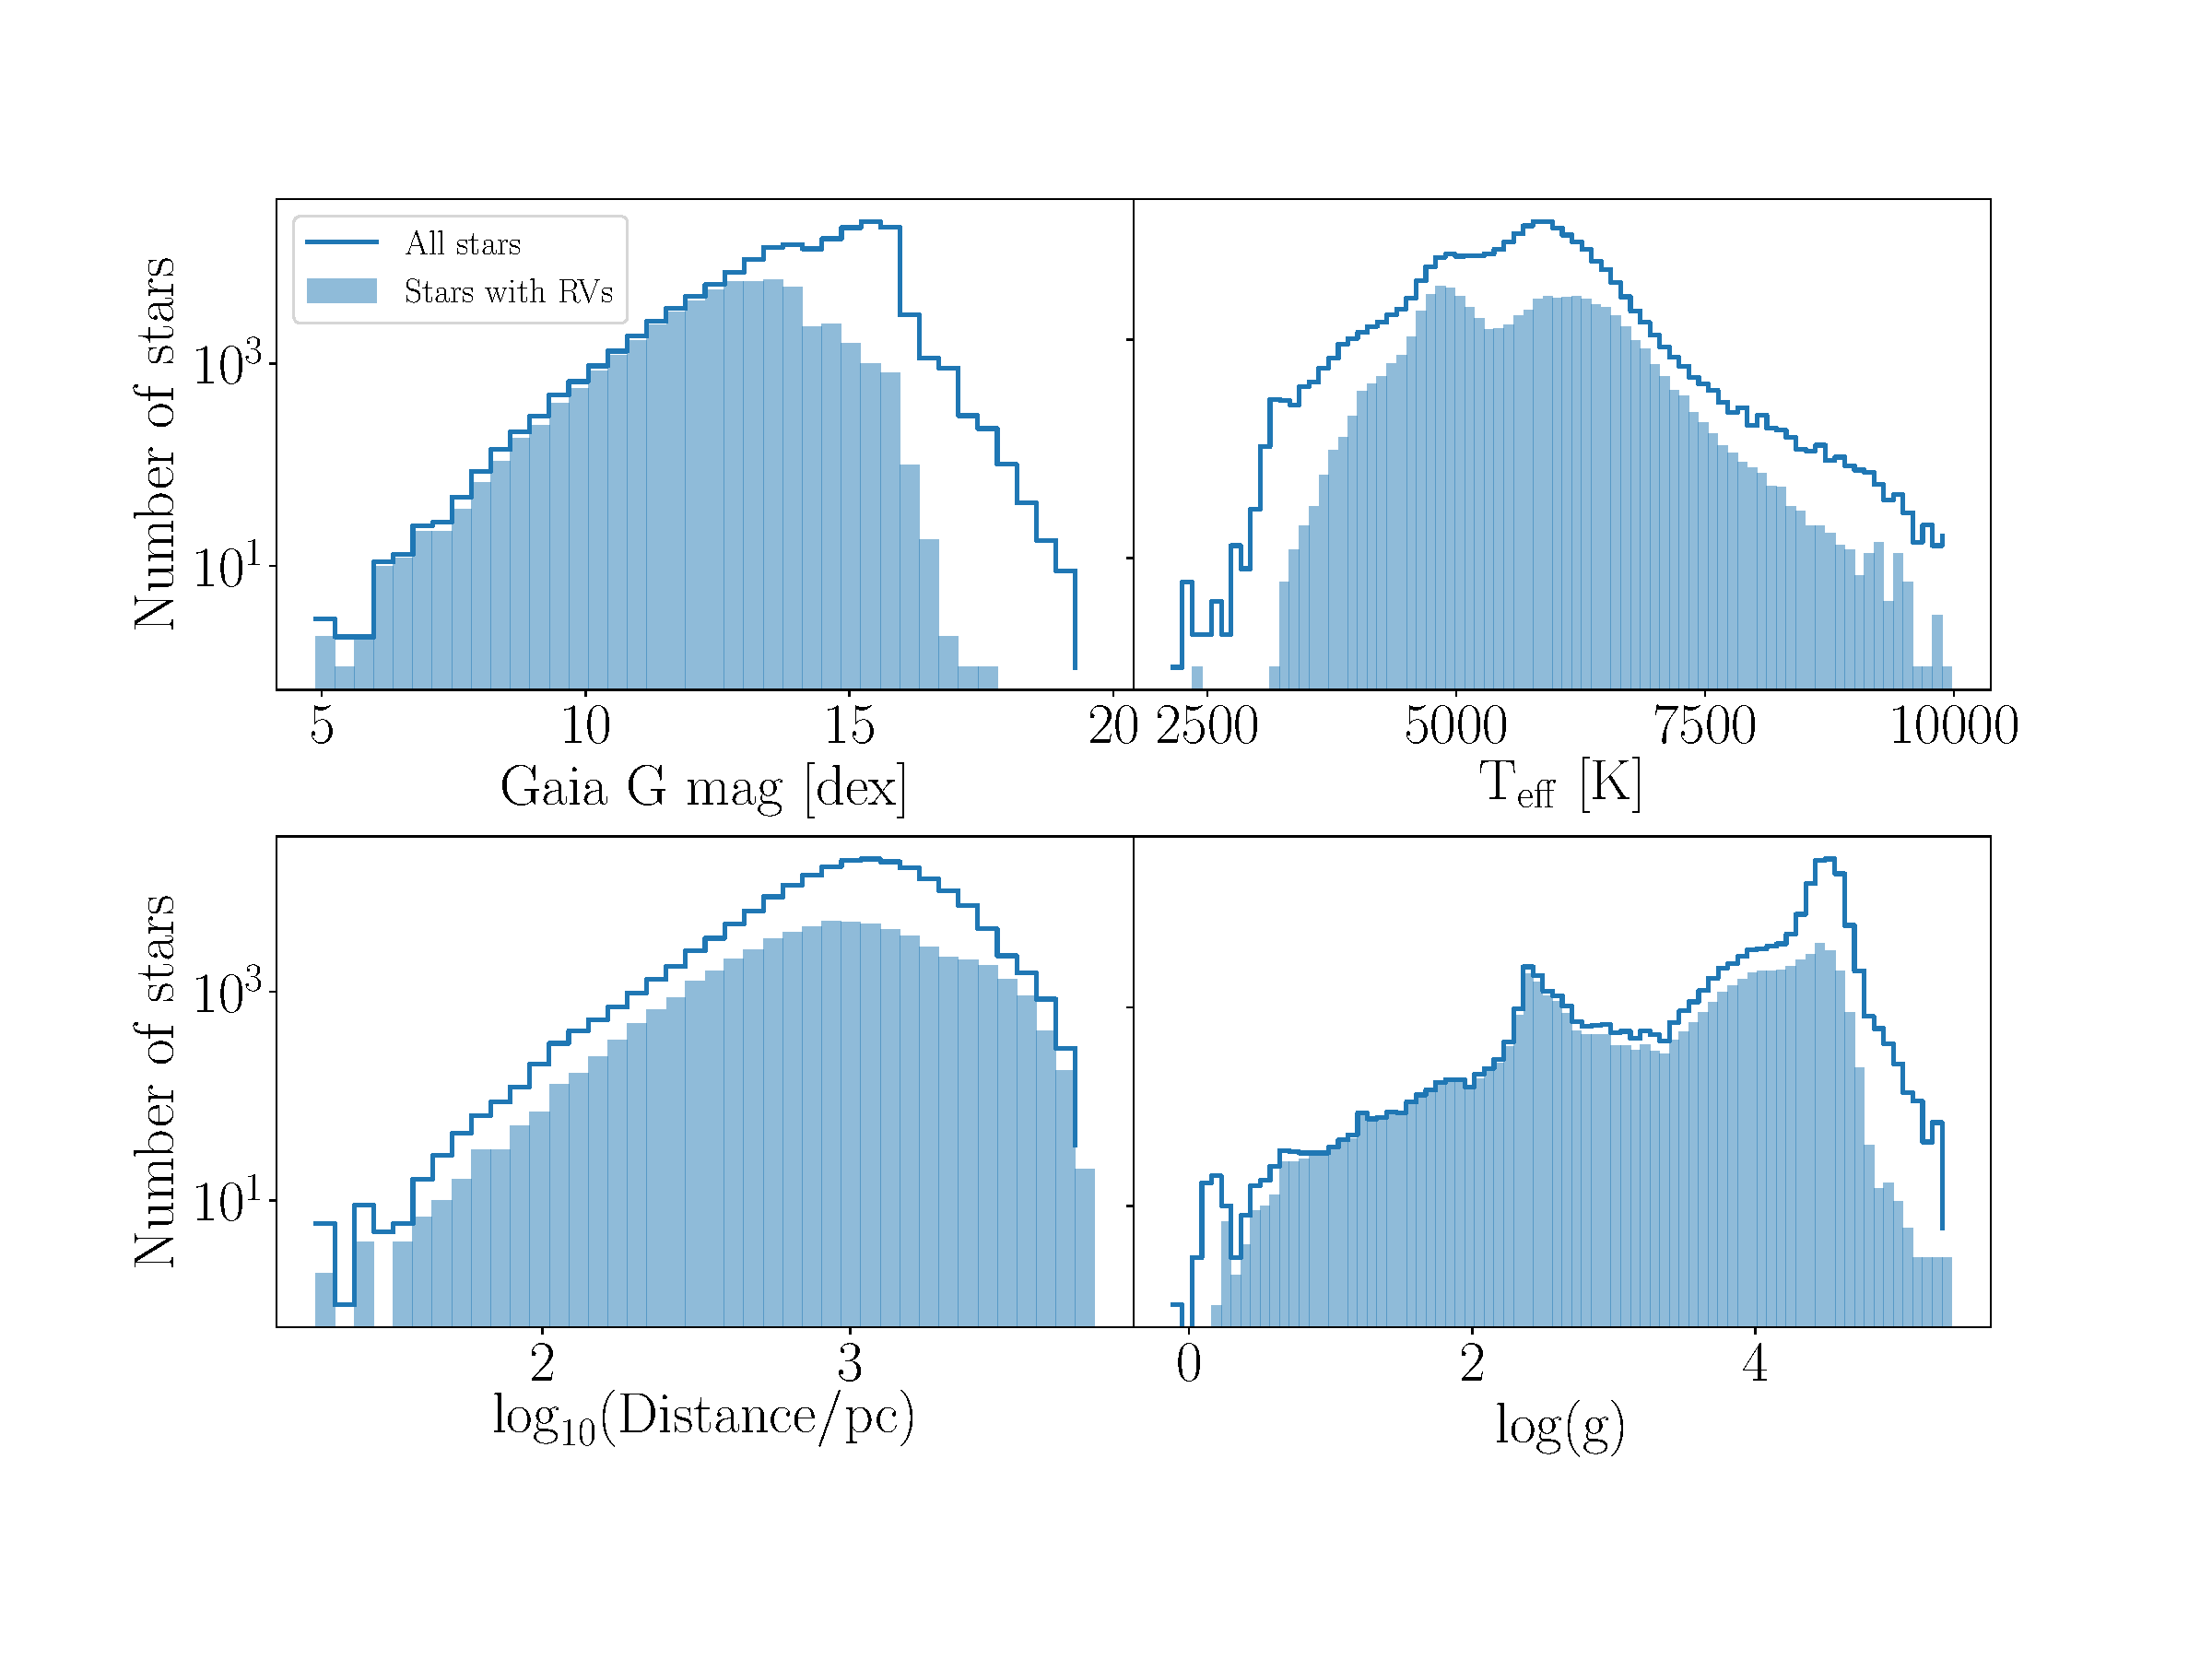
\includegraphics[width=1\textwidth]{rv_histogram}
\label{fig:rv_histogram}
\end{figure}
Given that rotational evolution is particularly poorly understood for M
dwarfs, the cool stars with missing RVs are arguably the most interesting.
To fill-in the low-temperature regime, we inferred velocities for stars
without RV measurements, by marginalizing over missing RVs.
